\section{Бутстреп оценка 0.632}
Простую бутстреп оценку (17.17) можно записать иначе: 
\begin{equation}
\mathrm{E}_{\what{\text{F}}}[\text{err}(\textbf{x}^{*}, \what{\text{F}})] = \frac{1}{B\cdot n} \sum_{b = 1}^{B} \sum_{i = 1}^{n} \mathcal{Q}[y_{i},  \eta_{\textbf{x}^{*b}}(\textbf{c}_{i})].
\end{equation}
Мы можем рассматривать уравнение (17.22) как оценку ошибки прогноза для каждой точки данных $(\textbf{c}_{i}, y_{i})$, а затем усреднение ошибки по $i = 1, 2, ... n$. Теперь для кждого наблюдения $(\textbf{c}_{i}, y_{i})$ можно разделить бутстреп выборки на те, которые содержат наблюдение $(\textbf{c}_{i}, y_{i})$, и те, которые его не содержат. Ошибка предсказания для наблюдения $(\textbf{c}_{i}, y_{i})$, будет больше для бутстреп выборки, которая его не содержит, поскольку такая бутстреп выборка в некотором смысле <<дальше>> от наблюдения $(\textbf{c}_{i}, y_{i})$. Идея, лежащая в основе бутстреп оценки 0.632, состоит в том, чтобы использовать ошибку предсказания для корректировки <<оптимизма>> в явной частоте ошибок только для таких ситуаций.

Пусть $\epsilon_{0}$ будет средней частотой ошибок, полученной из бутстреп наборов данных, не содержащих прогнозируемое наблюдение (ниже мы приводим подробные сведения об оценке $\epsilon_{0}$). Как и раньше, $\text{err}(\textbf{x}, \what{\text{F}})$ --- это явная частота ошибки. Разумным выглядит использование нескольких $\epsilon_{0}$ - $\text{err}(\textbf{x}, \what{\text{F}})$ как <<оптимизм>> оценку  $\text{err}(\textbf{x}, \what{\text{F}})$. <<оптимизм>> оценка $0.632$ определяется как:
\begin{equation}
\what{\omega}^{0.632} = 0.632[\epsilon_{0} - \text{err}(\textbf{x}, \what{\text{F}})].
\end{equation}
Прибавление этой оценки к $\text{err}(\textbf{x}, \what{\text{F}})$ дает оценку ошибки предсказания 0.632:
\begin{equation}
\begin{gathered}
\what{\text{err}}^{0.632} = \text{err}(\textbf{x}, \what{\text{F}}) + 0.632[\epsilon_{0} - \text{err}(\textbf{x}, \what{\text{F}})] = \\
= 0.368 \cdot \text{err}(\textbf{x}, \what{\text{F}}) + 0.632 \cdot \epsilon_{0}.
\end{gathered}
\end{equation}

Аргумент <<0.632>> возникает из теоретического факта, который показывает что бутстреп выборки, используемые при вычислении $\epsilon_{0}$, в среднем дальше, чем типичный тестовый образец, примерно в $1 / 0.632$ раза. Корректировка в (17.23) исправляет это, поэтому $\what{\text{err}}^{0.632}$ примерно несмещенно для истинной частоты ошибки. Мы не будем приводить здесь теоретические факты, но отметим, что значение $0.632$ возникает потому, что это приблизительная вероятность того, что данное наблюдение появится в бутстреп выборке размера $n$.

С учетом B бутстреп выборк, мы можем оценить $\epsilon_{0}$ как:
\begin{equation}
\epsilon_{0} = \frac{1}{n}\sum_{i = 1}^{n} \sum_{b \in C_{i}} \frac{ \mathcal{Q}[y_{i},  \eta_{\textbf{x}^{*b}}(\textbf{c}_{i})] }{B_{i}},
\end{equation}
где $C_{i}$ --- это набор индексов бутстреп выборок, не содержащих $i$-ое наблюдение, а $B_{i}$ --- количество таких бутстреп выборок. В таблице 17.2 показыны номера наблюдений, которые появляются в каждой из 10 бутстреп выборок таблицы 17.1. Например, наблюдение $№ 5$ не появляется в бутстреп выборках 3, 4, 8 и 9. В обозначениях уравнения (17.25) $C_{i} = (3, 4, 8, 9)$. Таким образом, мы будем использовать только эти четыре бутстреп выборки для оценки ошибки предсказания для $i = 5$ наблюдения в уравнении (17.25).

В нашем примере $\epsilon_{0}$ равно $3.63$. Неудивительно, что она больше, чем явная ошибка, равная 2.20, поскольку это средняя ошибка предсказания для наблюдений, которых нет в бутстреп выборке, которая используется для их предсказания. Следовательно, оценка ошибки предсказания $0.632$ равна $0.368 \cdot 2.20 + 0.632 \cdot 3.63 = 3.10$, что близко к значению $3.00$, которое было получено ранее с помощью улучшенного бутстреп подхода. 

\begin{figure}[h]
\center{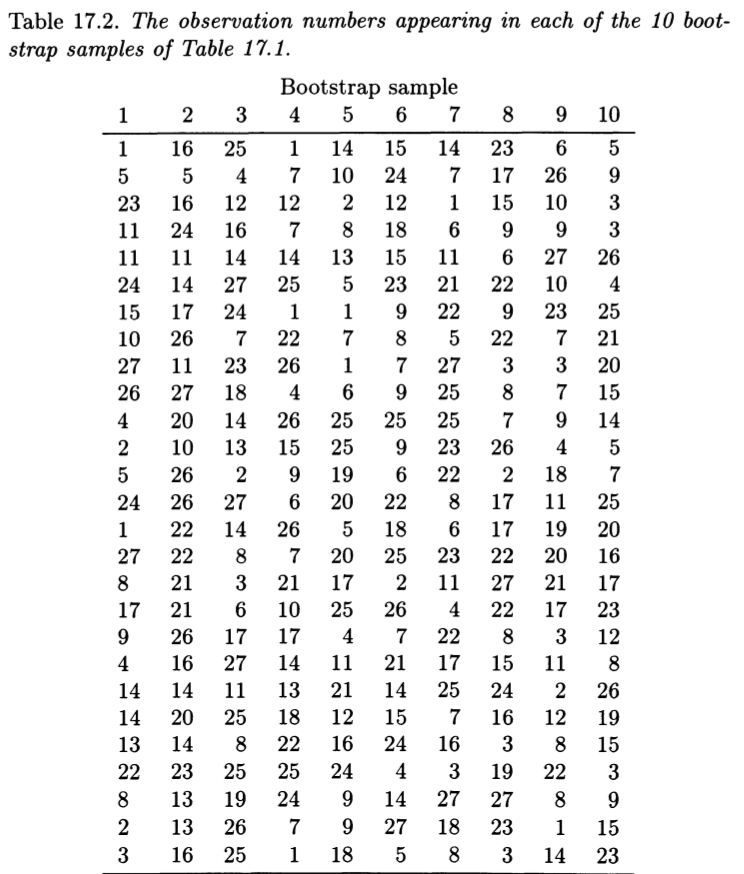
\includegraphics[width=1 \linewidth]{17/t17.7.1.png}}
\end{figure}
Интересно отметить, что средняя ошибка предсказания для наблюдений, которые присутствовали в бутстреп выборке, которая использовалась для их предсказания, составляла $3.08$, однако, это значение не используется при построении оценки $0.632$.